\documentclass[../EDI_Task4_Karwowski_Kowalewski.tex]{subfiles}

\begin{document} {

    Do badań i eksperymentów zostały wykorzystane następujące obrazy:
    \begin{figure}[!htbp]
        \begin{minipage}[c]{0.49\linewidth}
            \centering
            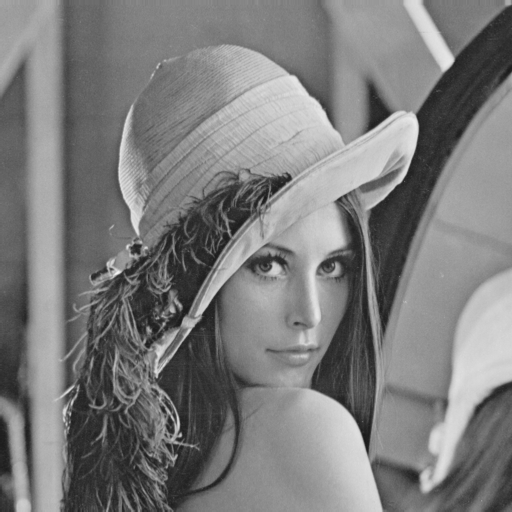
\includegraphics[width=0.75\textwidth]{img/original/01.png}
            \caption{Obraz 01.bmp}
        \end{minipage}\hfill
        \begin{minipage}[c]{0.49\linewidth}
            \centering
            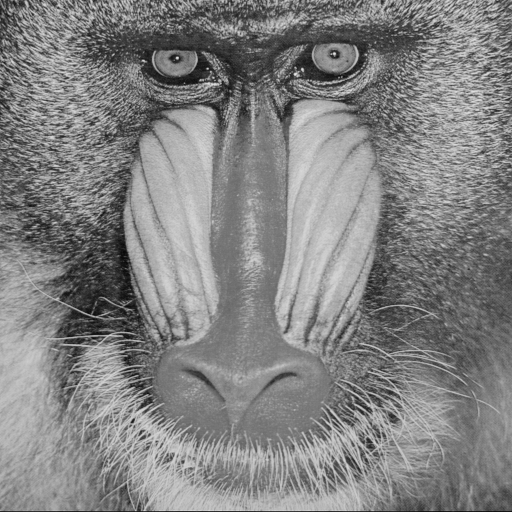
\includegraphics[width=0.75\textwidth]{img/original/02.png}
            \caption{Obraz 02.bmp}
        \end{minipage}
    \end{figure}

    \begin{figure}[!htbp]
        \begin{minipage}[c]{0.49\linewidth}
            \centering
            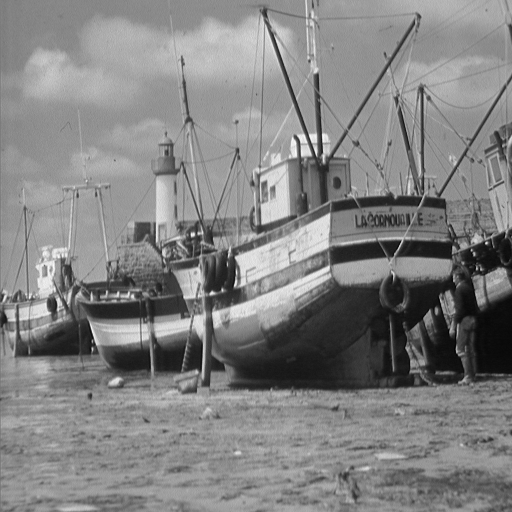
\includegraphics[width=0.75\textwidth]{img/original/03.png}
            \caption{Obraz 03.bmp}
        \end{minipage}\hfill
        \begin{minipage}[c]{0.49\linewidth}
            \centering
            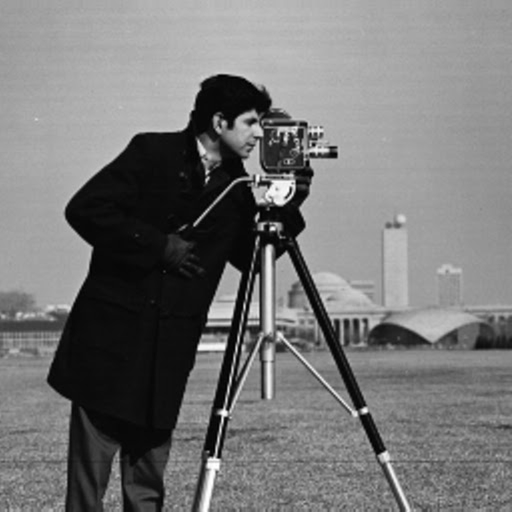
\includegraphics[width=0.75\textwidth]{img/original/04.png}
            \caption{Obraz 04.bmp}
        \end{minipage}
    \end{figure}

    \begin{figure}[!htbp]
        \begin{minipage}[c]{0.49\linewidth}
            \centering
            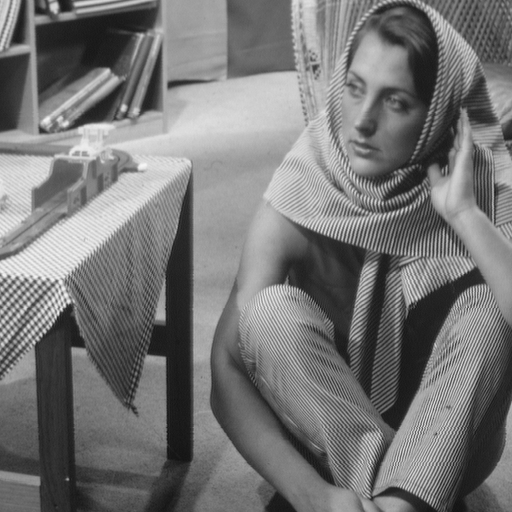
\includegraphics[width=0.75\textwidth]{img/original/05.png}
            \caption{Obraz 05.bmp}
        \end{minipage}\hfill
        \begin{minipage}[c]{0.49\linewidth}
            \centering
            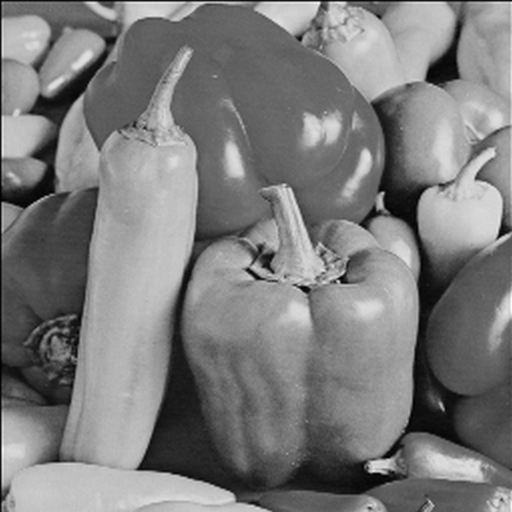
\includegraphics[width=0.75\textwidth]{img/original/06.png}
            \caption{Obraz 06.bmp}
        \end{minipage}
    \end{figure}

    \begin{figure}[!htbp]
        \begin{minipage}[c]{0.49\linewidth}
            \centering
            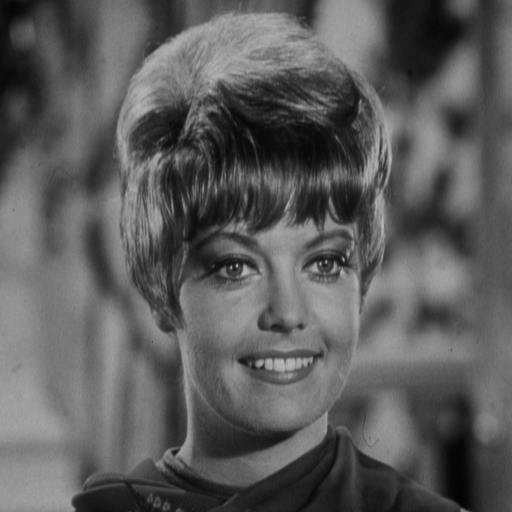
\includegraphics[width=0.75\textwidth]{img/original/07.png}
            \caption{Obraz 07.bmp}
        \end{minipage}\hfill
        \begin{minipage}[c]{0.49\linewidth}
            \centering
            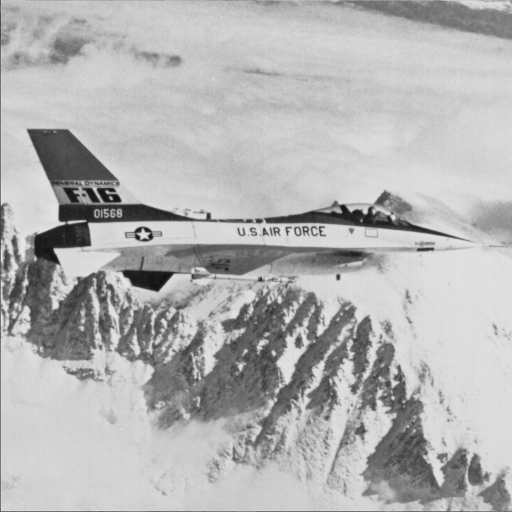
\includegraphics[width=0.75\textwidth]{img/original/08.png}
            \caption{Obraz 08.bmp}
        \end{minipage}
    \end{figure}
    \FloatBarrier

    Dla wszystkich eksperymentów zostały ustawione nastepujące parametry:
    \begin{itemize}
        \item \textbf{(--neurons\_sequence)} = 4 8 16 32
        \item \textbf{(--iterations)} = 10000
        \item \textbf{(--learning\_rate)} = 0.01
        \item \textbf{(--patterns\_number)} = 10000
        \item \textbf{(--pattern\_width)} = 8
    \end{itemize}
    Jedynymi zmiennymi parametrami były obrazy treningowe. Zawsze były wybierane dwa i
    w każdym eksperymencie zostały wskazane ich numery.
}
\end{document}
